\newpage
\section{Regresión Lineal}
\subsection{Enunciado}
\textbf{A:} Completar la segunda parte del modelo lineal presentado en clases.
\begin{figure}[h!]
    \centering
    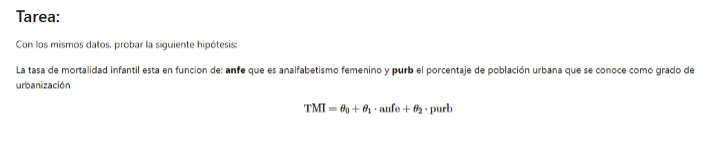
\includegraphics[width=1\textwidth]{images/statement.png}
    \caption{Enunciado de regresión lineal}
    \label{fig:regresion_lineal_statement}
\end{figure}

\textbf{B:} Generar una regresión lineal múltiple con 3 variables: dos  independiente y 1 dependientes (variable target, objetivo). Puede usar las bases de datos reales que uso en las prácticas anteriores.